\documentclass[uplatex,dvipdfmx,a4paper,10pt,fleqn]{jsarticle}

\input{preamble.tex}

%inputなどのプリアンブルを無視
\usepackage{docmute}


\usepackage{fancyhdr}
\pagestyle{fancy}
\lhead{}
\chead{理工系の微分積分・解答集}
\rhead{\thepage}
\cfoot{}


\begin{document}
\title{ \normalsize \textsc{}
		\\ [2.0cm]
		\HRule{1.5pt} \\
		\huge {\uppercase{理工系の微分積分学・解答集}
		\HRule{2.0pt} \\ [0.6cm] \LARGE{2023.8〜} \vspace*{10\baselineskip}}
		}
\date{}
\author{\LARGE なまちゃん}
\maketitle

\newpage 
\begin{multicols*}{3}
    \tableofcontents
\end{multicols*}
\addcontentsline{toc}{section}{\texorpdfstring{目次}{目次}}
\newpage
\section*{第1章:極限と連続性}
\addcontentsline{toc}{section}{\texorpdfstring{第1章:極限と連続性}{第1章:極限と連続性}}

\subsection*{p3:問1}
\addcontentsline{toc}{subsection}{\texorpdfstring{p3:問1}{p3:問1}}

\begin{tleftbar}
    \begin{proof}
        まず,$\abs{x}$,$\abs{y}$の定義により,
        \[
            -\abs{x} \leqq x \leqq  \abs{x},\quad -\abs{y} \leqq y \leqq  \abs{y}
        \]
        が成り立つ.この2式の辺々を足して,
        \[
            -(\abs{x}+\abs{y}) \leqq x+y \leqq \abs{x}+\abs{y}
        \]
        を得る.さらに,
        \[
            \abs{x} + \abs{y} \geqq \max \{ x+y , -(x+y) \} = \abs{x+y}
        \]
        となる.また,
        \begin{align*}
           &  \abs{x}= \abs{x-y +y} \leqq \abs{x-y} +\abs{y} \\
           & \therefore ~ \abs{x} - \abs{y} \leqq \abs{x-y}
        \end{align*}
        となる.$x \geqq y$,$x \leqq y$のときがあることを加味すると,
        \[
            \abs{\abs{x} - \abs{y}} \leqq \abs{x \pm y} 
        \]
        である.以上より,
        \[
            \abs{\abs{x} - \abs{y}} \leqq \abs{x \pm y} \leqq \abs{x}+\abs{y}
        \]
        が成り立つことが示された.
    \end{proof}
\end{tleftbar}


\subsection*{p3:問2}
\addcontentsline{toc}{subsection}{\texorpdfstring{p3:問2}{p3:問2}}

\begin{tleftbar}
    \begin{proof}
       $n$に関する数学的帰納法で証明する.
       \begin{enumerate}[(I)]
        \item $n=1$のとき,
        \[
            (1+x)^1 = 1+x
        \]
        により,与えられた等式は成り立つ.
        \item $n=k$としたときに,与えられた等式が成り立つと仮定すると,
        \[
            (1+x)^k \geqq 1+ kx + \frac{k(k-1)}{2} x^2 
        \]
        が成り立つ.この式の両辺に$(1+x)$をかけ,
        \begin{align*} 
            (1+x)^{k+1}  & \geqq \left ( 1+ kx + \frac{k(k-1)}{2} x^2 \right ) (1+x) \\
            & = 1+(k+1)x + \frac{k(k+1)}{2} x^2 + \frac{k(k-1)}{2} x^3 \\
            & \geqq 1+(k+1)x + \frac{k(k+1)}{2} x^2 
        \end{align*}
        であるから,$n =k+1$のときにもこの等式は成り立つ.
       \end{enumerate}
       (I),(II)の考察により証明された.
    \end{proof}
\end{tleftbar}

\newpage 



\subsection*{p5:問3}
\addcontentsline{toc}{subsection}{\texorpdfstring{p5:問3}{p5:問3}}

\begin{tleftbar}
    \begin{proof}
        必要性,十分性をそれぞれ示す.
        \begin{enumerate}[(I)]
            \item 必要性について示す.$m \coloneqq \max E$とすると.任意の$ x \in E$について$x \leqq m$である.よって$m$は$E$の上界のひとつである.
            また,$m \in E$より,$l$を$E$の上界とすると,$m \le l$である.よって$m$は$E$の上界の最小数であり,上限の定義により$\sup E = m \in E$となる.
            \item 十分性について示す.$\alpha$は$E$の上界の最小元だから,$E$の任意の元$x$について$x \le \alpha $.一方$\alpha  \in E$でもあるから$\max E = \alpha$となり$E$は最大値をもつ.
        \end{enumerate}
        以上(I),(II)により示された.
    \end{proof}
    \end{tleftbar}


    \subsection*{p5:問4-(1)}
    \addcontentsline{toc}{subsection}{\texorpdfstring{p5:問4-(1)}{p5:問4-(1)}}

    \begin{tleftbar}
        $A \coloneqq \{ 1 + 1/n \mid n \in \mathbb{N} \}$,$ a_n \coloneqq 1+1/n$とする.

        任意の$n \in \mathbb{N}$に対して,$a_{n+1} \leqq a_n$であることにより,$\{ a_n \}$は単調減少列である.ゆえに
        \[
            \sup A = a_1 = 2
        \]
        である.
        
        下限については
        \[
            \lim_{n \to \infty} \left ( 1 + \frac{1}{n} \right) = 1
        \]
        であることと,$\{ a_n \}$はその下限に収束することにより,
        \[
            \inf A = 1 
        \]
        となる.
        
        以上により,
        \[
            \sup \{ 1 + 1/n \mid n \in \mathbb{N} \} = 2 , \quad \inf \{ 1 + 1/n \mid n \in \mathbb{N} \}=1
        \]
        である.
    \end{tleftbar}


    \subsection*{p5:問4-(2)}
    \addcontentsline{toc}{subsection}{\texorpdfstring{p5:問4-(2)}{p5:問4-(2)}}

    \begin{tleftbar}
        数列$\{ a_n \}$は単調増加数列であることにより,$\{ a_n \}$の定義から,
        \[
            \lim_{n \to \infty} a_n = \pi 
        \]
        となることと併せると,$\sup \{ a_n \mid n \in \mathbb{N} \} = \pi$である.
        
        他方,任意の$n \in \mathbb{N}$に対して,$ a_n \geqq a_1 = 3.1$であることにより,
        \[
            \inf \{ a_n \mid n \in \mathbb{N} \} =3.1
        \]
        である.

        以上の考察により,
        \[
            \sup \{ a_n \mid n \in \mathbb{N} \} = \pi,\quad    \inf \{ a_n \mid n \in \mathbb{N} \} =3.1
        \]
        である.
    \end{tleftbar}




    \subsection*{p7:問6}
    \addcontentsline{toc}{subsection}{\texorpdfstring{p7:問6}{p7:問6}}

    \begin{tleftbar}
        \begin{proof}
            与えられた条件により,任意の$\varepsilon>0$に対して,$N_1 \in \mathbb{N}$が存在して,任意の$n \in \mathbb{N}$に対して,
    \[
        n \geqq N_1 \Longrightarrow \abs{\frac{1}{a_n}-0}<\varepsilon
    \]
    が成り立つ,ここで$M \coloneqq \frac{1}{\varepsilon}$とおくと,上の$N_1 \in \mathbb{N}$に対して,
    \[
        n \geqq n_0 \Longrightarrow a_n  >\frac{1}{\varepsilon}=M
    \]
    となり,これより$\lim_{n \to \infty} a_n=\infty$が示された.

    さて,$\lim_{n \to \infty} a_n = \infty$を仮定すると,
        任意の$M>0$に対して,$N_2 \in \mathbb{N}$が存在して,任意の$n \in \mathbb{N}$に対して,
        \[
            n \geqq N_2 \Longrightarrow a_n > M
        \]
        が成り立つ.

        ここで$\varepsilon \coloneqq  1/M$とすると,

        \[
            n \geqq N_2 \Longrightarrow 0< \frac{1}{a_n} < \frac{1}{M}= \varepsilon 
        \]
        となり$\lim_{n \to \infty} 1/a_n = 0$となる.
        
        以上の考察により証明された.
        \end{proof}
        \end{tleftbar}

        \subsection*{p7:問7}
        \addcontentsline{toc}{subsection}{\texorpdfstring{p7:問7}{p7:問7}}
    
\begin{leftbar} \begin{proof}
    任意の$M > 0$に対し,
    \[
      a_n > M + 1 \quad (n > N)
    \]
    なる$N$が存在する.
    $m > \max \left\{ N, N(M + 1) - \sum_{k = 1}^N a_k \right\}$となるような$m$をひとつとり固定する.
    $n > m$に対して
    \begin{align*}
      b_n
      &= \frac{1}{n} \sum_{k = 1}^N a_k + \frac{1}{n} \sum_{k = N + 1}^n a_k \\
      &> \frac{N(M + 1) - n}{n} + \frac{n - N}{n} (M + 1) \\
      &= M
    \end{align*}
  \end{proof}
\end{leftbar}
  
  \newpage
 
    \subsection*{p9:問8}
    \addcontentsline{toc}{subsection}{\texorpdfstring{p9:問8}{p9:問8}}

    \begin{tleftbar}
        \begin{proof}
        与えられた式から,任意の$\varepsilon >0$に対して,$N_1 , N_2 \in \mathbb{N}$が存在して,
        任意の$n \in \mathbb{N}$に対して,
        \begin{align*} 
            & n \geqq N_1 \Longrightarrow \abs{a_n - \alpha}<\varepsilon \\
            & n \geqq N_2 \Longrightarrow \abs{b_n - \beta}<\varepsilon 
        \end{align*} 
        となる.

        さて,$N_3 \coloneqq \max \{ N_1 , N_2 \}$とすると,
        \[
           n \geqq N_3  \Longrightarrow \abs{(a_n+b_n)-(\alpha + \beta) } \leqq  \abs{a_n - \alpha}+\abs{b_n-\beta}<\varepsilon +\varepsilon=2\varepsilon 
         \]
         となり,
         \[
            \lim_{n \to \infty} (a_n + b_n)= \alpha + \beta
         \]
         を得る.

         後半についても,上の$N_1$,$N_2$,$N_3$を用いて証明する.

         さて,$\{ a_n \}$と$\{ b_n \}$は収束するので,有界であることがわかり,ある$M$が存在して,任意の$n \in \mathbb{N}$に対して,
         \begin{align*} 
            &\abs{a_n} \leqq M \\
            & \abs{b_n} \leqq M 
         \end{align*} 
         である.よって,$n \geqq N_3$のとき,
         \begin{align*} 
            \abs{a_n b_n - \alpha \beta} & \leqq \abs{b_n} \abs{a_n -\alpha } + \abs{\alpha} \abs{b_n -\beta} \\
            & < (M+\alpha )\varepsilon 
         \end{align*} 
         となるため,
         \[
            \lim_{n \to \infty} a_n b_n = \alpha \beta
         \]
         が成り立つ.

         以上の考察により証明された.
        \end{proof}
        \end{tleftbar}



    \subsection*{p9:問9-(1)}
    \addcontentsline{toc}{subsection}{\texorpdfstring{p9:問9-(1)}{p9:問9-(1)}}

    \begin{tleftbar}
        \begin{proof}
        $\{ a_n \}$と$ \{ a_n + b_n \}$が収束するので,任意の$\varepsilon >0$に対して,ある$N_1 , N_2 \in \mathbb{N}$が存在して,
        任意の$n \in \mathbb{N}$に対して,
        \begin{align*} 
            &n \geqq N_1 \Longrightarrow \abs{a_n - \alpha}<\varepsilon \\
            & n \geqq N_2 \Longrightarrow \abs{(a_n + b_n)-\gamma}<\varepsilon 
        \end{align*} 
        が成立する.

        さて,$N_3 \coloneqq \max \{ N_1 , N_2 \}$とすると,$n \geqq N_3$のとき,
        \begin{align*} 
            \abs{b_n - (\gamma - \alpha )} & \leqq  \abs{(a_n+b_n)-\gamma} + \abs{\alpha - a_n} \\
            & < \varepsilon + \varepsilon = 2 \varepsilon 
        \end{align*}
        となり,数列$\{b_n \}$は$\gamma - \alpha $に収束する.
    \end{proof}
    \end{tleftbar}


    \subsection*{p9:問9-(2)}
    \addcontentsline{toc}{subsection}{\texorpdfstring{p9:問9-(2)}{p9:問9-(2)}}


 \begin{leftbar} \begin{proof}
    $a_n b_n \to \gamma$とする.
    任意の$\varepsilon > 0$をとる.
    $a_n \to \alpha$から$\frac{1}{a_n} \to \frac{1}{\alpha}$ ($\because$ Thm2)
    \begin{enumerate}[label = (\roman*)]
      \item $\gamma \ne 0$のとき,仮定より
            \[
              \abs{\frac{1}{a_n} - \frac{1}{\alpha}} < \frac{\varepsilon}{2 \lvert \gamma \rvert} \quad (n \geq N_1)
            \]
            \[
              \abs{a_n b_n - \gamma} < \frac{\varepsilon}{2 \left( 1 + \frac{1}{\abs{\alpha}} \right)} \quad (n \geq N_2)
            \]
            となる$N_1, N_2$が存在する.
            このとき,$N = \max \{ N_1, N_2 \}$とすると,
            \begin{align*}
              \abs{b_n - \frac{\gamma}{\alpha}}
              &= \abs{\frac{1}{a_n}(a_n b_n - \gamma) + \gamma \left( \frac{1}{a_n} - \frac{1}{\alpha} \right)} \\
              &\leq \abs{\frac{1}{a_n}} \abs{a_n b_n - \gamma} + \abs{\gamma} \abs{\frac{1}{a_n} - \frac{1}{\alpha}} \quad (n \geq N) \; \cdots \; (*)
            \end{align*}
            ここで,$\abs{\frac{1}{a_n} - \frac{1}{\alpha}} < 1 \quad (n \geq N_3)$となる$N_3$が存在し,
            \[
              \abs{\frac{1}{a_n} - \frac{1}{\alpha}} \geq \abs{\frac{1}{a_n}} - \abs{\frac{1}{\alpha}}
            \]
            から,
            \[
              \abs{\frac{1}{a_n}} < 1 + \frac{1}{\abs{\alpha}}
            \]
            よって,$N' := \max\{ N_1, N_2, N_3 \}$とすれば,
            \begin{align*}
              \abs{b_n - \frac{\gamma}{\alpha}}
              &\leq \frac{1}{\abs{a_n}} \abs{a_n b_n - \gamma} + \abs{\gamma} \abs{\frac{1}{a_n} - \frac{1}{\alpha}} \\
              &< \left( 1 + \frac{1}{\abs{\alpha}} \right) \frac{\varepsilon}{2 \left( 1 + \frac{1}{\abs{\alpha}} \right)} + \abs{\gamma} \cdot \frac{\, \frac{\varepsilon}{2} \,}{\abs{\gamma}} \\
              &= \frac{\varepsilon}{2} + \frac{\varepsilon}{2} \\
              &= \varepsilon \quad (n \geq N')
            \end{align*}
      \item $\gamma = 0$のとき
            \begin{align*}
              \abs{b_n - 0}
              &= \abs{\frac{1}{a_n}} \abs{a_n b_n} \\
              &< \left( 1 + \frac{1}{\abs{\alpha}} \right) \cdot \frac{\varepsilon}{2 \left( 1 + \frac{1}{\abs{\alpha}} \right)} \\
              &< \varepsilon
            \end{align*}
            より$b_n \to 0$
    \end{enumerate}
  \end{proof}
\end{leftbar}

\newpage 


    \subsection*{p9:問10}
    \addcontentsline{toc}{subsection}{\texorpdfstring{p9:問10}{p9:問10}}
    

\begin{tleftbar}
    \begin{proof}
        $a>b$であると仮定する.このとき,$a-b >0$なので,$a-b=2 \varepsilon$とおくと,ある$N \in \mathbb{N}$が存在して,任意の$n \in \mathbb{N}$に対して,
        \[
            n \geqq N \Longrightarrow \abs{a_n -a} < \varepsilon
        \]
        \[
            n \geqq n_0 \Longrightarrow \abs{b_n -b} <\varepsilon
        \]
        が成立.このような$n \in \mathbb{N}$に対し,
        \[
            b_n< b+\varepsilon = a-\varepsilon < a_n
        \]
        となるが,これは矛盾である.
        
        よって先の仮定が誤りであり,ここまでで前半の主張が示された.

        後半については,$\lim_{n \to \infty} a_n = \infty$から,
        任意の$M >0$に対して,ある$N \in \mathbb{N}$が存在して,任意の$n \in \mathbb{N}$に対して
        \[
            n \geqq N \Longrightarrow a_n >M 
        \]
        が成り立つ.このとき,$a_n \leqq b_n$なので,上の$N\in \mathbb{N}$に対して,
        \[
            n \geqq N \Longrightarrow b_n >M
        \]
        となり,このとき$\lim_{n \to \infty} b_n $となる.

        $\lim_{n \to \infty} b_n = -\infty$の場合も同様にして証明されるので,これで定理の主張が示された.
    \end{proof}
    \end{tleftbar}


    \subsection*{p10:問11}
    \addcontentsline{toc}{subsection}{\texorpdfstring{p10:問11}{p10:問11}}

    \begin{tleftbar}
        \begin{proof}
        数列$\{ a_n \}$を上に有界でない増加列とする.このとき,任意の実数$M$に対して,ある$N \in \mathbb{N}$があって,任意の$n \in \mathbb{N}$に対して,
        \[
            n \geqq N \Longrightarrow  M < a_N \leqq a_n
        \]
        となる.ゆえに
        \[
            \lim_{n \to \infty} a_n=\infty
        \]
        となり,これが証明すべきことであった.
        \end{proof}
    \end{tleftbar}
    
         
        \subsection*{p10:問12}
\addcontentsline{toc}{subsection}{\texorpdfstring{p10:問12}{p10:問12}}

\begin{tleftbar}
    $a=0$のときは明らかに$0$に収束するので,$a \ne 0$とする.$2\abs{a} \leqq N$となる$N \in \mathbb{N}$をとる.このとき,
    \begin{align*}
         0 &< \abs{ \frac{a^n}{n!} } \\
         &\leqq \frac{\abs{a}^n}{n!} \\
         &= \frac{\abs{a}^{N}}{N!} \cdot \frac{\abs{a}}{N+1} \cdot \frac{\abs{a}}{N+2} \dotsm \frac{\abs{a}}{n} \\
         & \leqq  \frac{\abs{a}^{N}}{N!} \left(\frac{1}{2} \right)^{n-N}
    \end{align*}
    であるから,
    \[
        - \frac{\abs{a}^{N}}{N!} \left(\frac{1}{2} \right)^{n-N} \leqq  \frac{a^n}{n!} \leqq \frac{\abs{a}^{N}}{N!} \left(\frac{1}{2} \right)^{n-N}
    \]
    となり,はさみうちの原理により,
    \[
        \lim_{n \to \infty} \frac{a^n}{n!} =0
    \]
    である
\end{tleftbar}

\newpage


\subsection*{p14:問13-(1)}
\addcontentsline{toc}{subsection}{\texorpdfstring{p14:問13-(1)}{p14:問13-(1)}}

\begin{tleftbar}
\[
   a_n = \frac{1}{n (n+1)(n+2)} = \frac{1}{2} \left ( \frac{1}{n(n+1)}- \frac{1}{(n+1)(n+2)} \right)
\]
とおく.$\{ a_n \}$の第$n$部分和を$S_n$とすると,
\begin{align*} 
    S_n & = \sum_{k=1}^{n}  \frac{1}{2} \left ( \frac{1}{k(k+1)}-\frac{1}{(k+1)(k+2)} \right) \\
    & = \frac{1}{4} - \frac{1}{2n(n+1)}
\end{align*} 
であるから,
\begin{align*}
    \lim_{n \to \infty} S_n &= \lim_{n \to \infty} \left (  \frac{1}{4} - \frac{1}{2n(n+1)} \right) \\
    &= \frac{1}{4}
\end{align*}
となるため,
\[
    \sum_{n=1}^{\infty} \frac{1}{n (n+1)(n+2)} = \frac{1}{4}
\]
である.
\end{tleftbar}


\subsection*{p14:問13-(2)}
\addcontentsline{toc}{subsection}{\texorpdfstring{p14:問13-(2)}{p14:問13-(2)}}

\begin{tleftbar}
    $a_n = \frac{n}{2^n}$とし,数列$\{ a_n \}$の第$n$部分和を$S_n$とすると,
    \[
        S_n = \frac{1}{2}+ \frac{2}{2^2}+\dots + \frac{n}{2^n}
    \]
    となる.これにより,
    \[
        \frac{1}{2} S_n = \frac{1}{2^2}+\frac{2}{2^3}+\dots + \frac{n}{2^{n+1}}
    \]
    となるため,
    \begin{align*} 
        & \frac{1}{2} S_n = \frac{1}{2}+ \frac{1}{2^2}  +\frac{1}{2^3}+\dots +\frac{1}{2^n}-\frac{n}{2^{n+1}} \\
       & \therefore ~ S_n = 2- \left (\frac{1}{2} \right)^{n-1} -\frac{n}{2^n}
    \end{align*} 
    となるため,
    \begin{align*}
        \lim_{n \to \infty} S_n &= \lim_{n \to \infty}\left ( 2- \left (\frac{1}{2} \right)^{n-1} -\frac{n}{2^n} \right ) \\
        & = 2
    \end{align*}
    である.よって
    \[
        \sum_{n=1}^{\infty} \frac{n}{2^n}=2
    \]
    となる.
\end{tleftbar}


\subsection*{p16:問14-(1)}
\addcontentsline{toc}{subsection}{\texorpdfstring{p16:問14-(1)}{p16:問14-(1)}}

\begin{tleftbar}
    \begin{proof}
    必要条件であること,十分条件であることをそれぞれ証明する.
    \begin{enumerate}[(I)]
        \item $\alpha$は$\{ a_n \}$の集積値であるから,$\{ a_n \}$の部分列で$\lim_{k\to \infty} a_{n(k)} = \alpha$となるような
        自然数列$\{ n (k) \}$が存在し,これよりただちに後半の主張が従う.
        \item 後半の条件のもと,$\abs{a_n - \alpha}< \varepsilon$となるような$n \in \mathbb{N}$が無限個存在するので,
        $1>0$に対し,$\abs{a_{n(1)}-\alpha}<1$となるような$n(1) \in \mathbb{N}$がある.
        このようにして,$\abs{a_{n(2)}-\alpha}< 1/2$となる$n(2) \in \mathbb{N}$を$n (1)<n(2)$となるようにとれる.
        この繰り返しで,自然数列$\{ n(k) \}$を
        \[
            \abs{a_{n(k)}-\alpha}< 1/k
        \]
        となるようにとることができ,$k \to \infty$としたときに$1/k \to 0$だから,これより$\alpha$が$\{ a_n \}$の集積値であることが従う.
    \end{enumerate}
    以上(I),(II)により証明された.
    \end{proof}
\end{tleftbar}


\subsection*{p16:問14-(3)}
\addcontentsline{toc}{subsection}{\texorpdfstring{p16:問14-(3)}{p16:問14-(3)}}

\begin{tleftbar}
    \begin{proof}
    必要条件であること,十分条件であることをそれぞれ証明する.
    \begin{enumerate}[(I)]
        \item $\lim_{n \to \infty} a_n = \alpha$とすると,$\{ a_n \}$の任意の部分列も$\alpha$に収束する.
        よって,上極限,下極限の定義により,
        \[
            \varlimsup_{n \to \infty} a_n = \varliminf_{n \to \infty} a_n = \alpha
        \]
        である.
        \item $ A_n =\{ k \in \mathbb{N} \mid k \geqq n \}$と定義すると
        \[
            \inf A_n \leqq a_n \leqq \sup A_n
        \]
        となる.

        いま仮定により,$\lim_{n \to \infty} \sup A_n = \lim_{n \to \infty} \inf A_n$であり,この値を$\alpha$とすると,
        はさみうちの原理により,
        \[
            \lim_{n \to \infty} a_n = \alpha
        \]
        となり,ただちに主張が従う.
    \end{enumerate}
    以上(I),(II)により証明された.
\end{proof}
\end{tleftbar}


\subsection*{p18:問21}
\addcontentsline{toc}{subsection}{\texorpdfstring{p18:問21}{p18:問21}}

\begin{tleftbar}
    \begin{proof}
    $ A = [0,1]$とする.

    $x \in A \setminus \mathbb{Q}$であるとき,$f(x)=1-x \in A \setminus \mathbb{Q}$ である.
    また,$x \in \mathbb{Q}$のとき,$f(x)=x \in \mathbb{Q}$である.

    次に,$ x_1 , x_2 \in A$となる$x_1$,$x_2$をとる.
    このとき
    \[
        f(x_1)=f(x_2)
    \]
    であると仮定する.このとき,上の考察により,$x_1 = x_2$もしくは$1-x_1 = 1-x_2$となり,いずれにせよ$x_1 =x_2$となる.

    よって,ここまでで$f$は一対一の写像であることが示された.
   
   さて, $ \sqrt{2}/2 \in A$,$7/10 \in A$であることは明らか.さらに,
    \[
        \left ( \frac{7}{10} \right)^2 = \frac{49}{100} <\frac{1}{2}=\left ( \frac{\sqrt{2}}{2} \right)^2 
    \]
    であるから,$7/10< \sqrt{2}/2$である.

    ここで,
    \[
    f\left ( \frac{7}{10} \right)=\frac{7}{10},\quad f\left(\frac{\sqrt{2}}{2} \right)= 1-\frac{\sqrt{2}}{2}
    \]
    であり.さらに
    \[
        1-\frac{\sqrt{2}}{2} <\frac{7}{10}
    \]
    なので,$f$は単調ではないことが示された.

    以上の考察により,$f$は一対一ではあるが単調ではない.
\end{proof}
\end{tleftbar}

\subsection*{p21:問24-(1)}
\addcontentsline{toc}{subsection}{\texorpdfstring{p21:問24-(1)}{p21:問24-(1)}}

\begin{tleftbar}
    計算すると,
    \begin{align*} 
        \lim_{x \to 0} \frac{\sin bx}{\sin ax} & = \lim_{x \to 0} \frac{\sin bx}{b x} \cdot \frac{ax}{ \sin ax} \cdot \frac{b}{a} \\
        & = 1 \cdot 1 \cdot \frac{b}{a} \\
        & = \frac{b}{a}
    \end{align*} 
    である.
\end{tleftbar}

\subsection*{p21:問24-(2)}
\addcontentsline{toc}{subsection}{\texorpdfstring{p21:問24-(2)}{p21:問24-(2)}}

\begin{tleftbar}
    $t = x - \pi/6$とおくと,
    \begin{align*} 
        \lim_{x \to \pi/6} \frac{\sin (2x-\pi/3)}{x - \pi/6} & = \lim_{t \to 0} \frac{\sin 2 t}{t} \\
        & = \lim_{t \to 0} \frac{\sin 2t}{2t} \cdot 2 \\
        & = 1 \cdot 2 \\
        & = 2 
    \end{align*} 
    である.
\end{tleftbar}




\subsection*{p23:問28-(1)}
\addcontentsline{toc}{subsection}{\texorpdfstring{p23:問28-(1)}{p23:問28-(1)}}

\begin{tleftbar}
    計算すると,
    \begin{align*} 
        \lim_{x \to \infty} \sqrt{x}(\sqrt{x+1}-\sqrt{x}) & = \lim_{x \to \infty} \frac{\sqrt{x}}{\sqrt{x+1}+\sqrt{x}} \\
        & = \frac{1}{1+1} \\
        & = \frac{1}{2}
    \end{align*}
    となる.
\end{tleftbar}


\subsection*{p32:3-(2)}
\addcontentsline{toc}{subsection}{\texorpdfstring{p32:3-(2)}{p32:3-(2)}}

\begin{tleftbar}
    \[
        a_n = \frac{1}{1 \cdot 2}+\frac{1}{2 \cdot 3} + \dots + \frac{1}{n(n+1)}
    \]
    とおくと,
    \begin{align*} 
       a_n & =  \sum_{k=1}^{n} \frac{1}{k(k+1)} \\
       & = \sum_{k=1}^{n} \left ( \frac{1}{k} - \frac{1}{k+1} \right ) \\
       & = 1-\frac{1}{n+1}
    \end{align*} 
    となり,
    \[
        \lim_{n \to \infty} a_n = \lim_{n \to \infty} \left ( 1-\frac{1}{n+1} \right) =1
    \]
    である.
\end{tleftbar}


\subsection*{p32:3-(3)}
\addcontentsline{toc}{subsection}{\texorpdfstring{p32:3-(3)}{p32:3-(3)}}

\begin{tleftbar}
    \[
        n \left ( \sqrt{1+\frac{1}{n}}-1 \right) = \sqrt{n^2+n}-n = \frac{n}{\sqrt{n^2+1}+n}
    \]
    であるから,これを$a_n$とすると,
    \begin{align*}
        \lim_{n \to \infty} a_n & =\lim_{n \to \infty}  \left ( \frac{n}{\sqrt{n^2+1}+n} \right) \\
        & = \frac{1}{2}
    \end{align*}
    となる.
\end{tleftbar}

\subsection*{p32:3-(4)}
\addcontentsline{toc}{subsection}{\texorpdfstring{p32:3-(4)}{p32:3-(4)}}

\begin{tleftbar}
\[
    3^n +n(-2)^n = 3^n \left (1+ \frac{n}{ \left (-\frac{3}{2} \right)^n } \right)
\]
なので,
\[
    \lim_{n \to \infty}  3^n \left (1+ \frac{n}{ \left (-\frac{3}{2} \right)^n } \right) =\infty
\]
により,
\[
    \lim_{n \to \infty} (3^n +n(-2)^n)=\infty 
\]
である.
\end{tleftbar}



\subsection*{p32:3-(5)}
\addcontentsline{toc}{subsection}{\texorpdfstring{p32:3-(5)}{p32:3-(5)}}

\begin{tleftbar}
    \[
        n \sin \frac{\pi}{n} = \frac{\sin (\pi/n)}{\pi/n} \cdot \pi 
    \]
    であり,
    \[
        \lim_{n \to \infty} \frac{\sin (\pi/n)}{\pi/n} \cdot \pi = 1 \cdot \pi =\pi
    \]
    なので,
    \[
        \lim_{n \to \infty} n \sin \frac{\pi}{n} = \pi
    \]
    である.
\end{tleftbar}




\subsection*{p32:5-(1)}
\addcontentsline{toc}{subsection}{\texorpdfstring{p32:5-(1)}{p32:5-(1)}}

\begin{tleftbar}
    $a>1$のとき,
    \begin{align*} 
        \lim_{n \to \infty} \frac{a^{n+1}}{a^n +1} & = \lim_{n \to \infty} \frac{a}{1+\dfrac{1}{a^n}} \\
        & = a 
    \end{align*} 
    となる.
    
    また,$0<a<1$のとき,
    \begin{align*} 
        \lim_{n \to \infty} \frac{a^{n+1}}{a^n +1} & = \frac{0}{0+1} \\
        & =0 
    \end{align*} 
    となる.

    また,$a=1$のとき,
    \begin{align*}
    \lim_{n \to \infty} \frac{a^{n+1}}{a^n +1} & = \frac{1}{1+1} \\
    & =\frac{1}{2}
    \end{align*}
    である.
\end{tleftbar}

\subsection*{p32:5-(2)}
\addcontentsline{toc}{subsection}{\texorpdfstring{p32:5-(2)}{p32:5-(2)}}

\begin{tleftbar} 
    $ 0 < a <1 $のとき,
    \begin{align*} 
        \lim_{n \to \infty} \frac{a^n - a^{-n}}{a^n + a^{-n}} & =\lim_{n \to \infty} \frac{a^{2n} - a^{0}}{a^{2n} + a^{0}} \\
        & = \frac{0-1}{0+1} \\
        & = -1 
    \end{align*} 
    である.

    $a=1$のとき
    \begin{align*}
    \lim_{n \to \infty} \frac{a^n - a^{-n}}{a^n + a^{-n}} & =  \lim_{n \to \infty} \frac{1-1}{1+1} \\
    & = 0
    \end{align*} 
    である.

    最後に,$a>1$のとき,
    \begin{align*} 
    \lim_{n \to \infty} \frac{a^n - a^{-n}}{a^n + a^{-n}} & =  \lim_{n \to \infty} \frac{a^0 - a^{-2n}}{a^0 + a^{-2n}} \\
    & = \frac{1-0}{1+0} \\
    & = 1 
    \end{align*}
    である.
\end{tleftbar}



\subsection*{p33:12-(1)}
\addcontentsline{toc}{subsection}{\texorpdfstring{p33:12-(1)}{p33:12-(1)}}

\begin{tleftbar}
    \begin{align*} 
        \lim_{x \to 0} \frac{e^{2x}-1}{e^{3x}-1} & = \lim_{x \to 0} \frac{e^{2x}-1}{2x} \cdot \frac{3x}{e^{3x}-1} \cdot \frac{2}{3} \\
        & = 1 \cdot 1 \cdot \frac{2}{3} \\
        & = \frac{2}{3}
    \end{align*} 
    となる.
\end{tleftbar}


\subsection*{p33:12-(2)}
\addcontentsline{toc}{subsection}{\texorpdfstring{p33:12-(2)}{p33:12-(2)}}

\begin{tleftbar}
    \[
        f(x)= (1+x+x^2)^{\frac{1}{x}}
    \]
    とおくと,
    \[
        \log f(x) = \frac{\log (1+x+x^2)}{x}
    \]
    となり,$\lim_{x \to 0} \log (1+x+x^2)=0$.$\lim_{x \to 0} x =0$であるから,ロピタルの定理を適用すると,
    \[
        \lim_{x \to 0} \frac{\log (1+x+x^2)}{x} =  \lim_{x \to 0}\frac{2x+1}{1+x+x^2} =1
    \]
    である.よって
    \[
        \lim_{x \to 0} f(x) = e^{1}=e
    \]
    となる.
\end{tleftbar}


\subsection*{p33:12-(3)}
\addcontentsline{toc}{subsection}{\texorpdfstring{p33:12-(3)}{p33:12-(3)}}

\begin{tleftbar}
    \[
        \log (x^{\frac{1}{1-x}})= \frac{\log x}{1-x}
    \]
    であり,$\lim_{x \to 1} \log x = 0$,$\lim_{x \to 1} (1-x)=0$であるから,
    ロピタルの定理が適用でき,
    \begin{align*} 
        \lim_{ x\to 1} \frac{\log x}{1-x} & = \lim_{x \to 1} \frac{1/x}{-1} \\
        & = \lim_{x \to 1} \left(-\frac{1}{x} \right ) \\
        & = -1 
    \end{align*}
    であるから,
    \begin{align*} 
        \lim_{x \to 1} x^{\frac{1}{1-x}} &= e^{-1} \\
        &= \frac{1}{e}
    \end{align*}
    である.
\end{tleftbar}


\subsection*{p33:12-(4)}
\addcontentsline{toc}{subsection}{\texorpdfstring{p33:12-(4)}{p33:12-(4)}}

\begin{tleftbar}
    まず,$\lim_{x \to 0} (1-\cos x)=0$,$\lim_{x \to 0} x^2 =0$であるから,ロピタルの定理が適用でき,
    \begin{align*} 
        \lim_{x \to 0} \frac{1-\cos x}{x^2} &= \lim_{x \to 0} \frac{\sin x}{2x} \\
        & = 1\cdot \frac{1}{2} \\
        & = \frac{1}{2}
    \end{align*} 
    となる.
\end{tleftbar}





\subsection*{p33:12-(6)}
\addcontentsline{toc}{subsection}{\texorpdfstring{p33:12-(6)}{p33:12-(6)}}

\begin{tleftbar}
    まず,
    \[
        -1 \leqq \sin \frac{1}{x} \leqq 1 
    \]
    である.これと$\abs{x} \geqq 0$であることから,
    \[
        -\sqrt{\abs{x}}\leqq \sqrt{\abs{x}} \sin \frac{1}{x} \leqq \sqrt{\abs{x}}
     \]
     を得る.ここで,$\lim_{x \to 0} (-\sqrt{\abs{x}})=0$,$\lim_{x \to 0} \sqrt{\abs{x}}=0$であることから,
     はさみうちの原理により,
     \[
        \lim_{x \to 0} \sqrt{\abs{x}} \sin \frac{1}{x} =0
     \]
     である.
\end{tleftbar}

\subsection*{p33:16-(1)}
\addcontentsline{toc}{subsection}{\texorpdfstring{p33:16-(1)}{p33:16-(1)}}

\begin{tleftbar} 
    計算すると,
    \begin{align*} 
        \cosh ^2 x - \sinh ^2 x & = \left ( \frac{e^x + e^{-x}}{2} \right)^2 - \left ( \frac{e^x - e^{-x}}{2} \right)^2 \\
        & = \frac{e^{2x}+2 + e^{-2x}}{4}- \frac{e^{2x}-2 + e^{-2x}}{4} \\
        & = \frac{4}{4} \\
        & =1 
    \end{align*} 
    である.
\end{tleftbar}



\subsection*{p34:22-(1)}
\addcontentsline{toc}{subsection}{\texorpdfstring{p34:22-(1)}{p34:22-(1)}}

\kakko{補題}

$\{ a_n \}$を実数列とする.このとき,
\[
    \lim_{n \to \infty} a_n =a
\]
であるならば,
\[
    \lim_{n \to \infty} \frac{a_1 + a_2 + \dots +a_n}{n} = a
\]
である.ただし$a$は実数の定数とする.

\begin{proof}
    $\lim_{n \to \infty} a_n =a$であるから,
    任意の$\varepsilon >0$に対して,ある$N_1 \in \mathbb{N}$が存在して,任意の$n \in \mathbb{N}$に対して,
    \[
        n \geqq N_1 \Longrightarrow \abs{a_n -a}<\varepsilon 
    \]
    となる.

    また,
    \[
        \abs{\frac{a_1+a_2+\cdots+a_n}{n}-a}= \abs{\frac{(a_1-a)+(a_2-a)+\cdots+(a_n-a)}{n}}
    \]
    と変形する.この右辺に補題を適用し,
    \[
        \abs{\frac{(a_1-a)+(a_2-a)+\cdots+(a_n-a)}{n}} \leqq \frac{\abs{a_1-a}+\abs{a_2-a}+\cdots+\abs{a_n-a}}{n}
    \]
    を得る.これにより,
    \[
        n \geqq N_1 \Longrightarrow \frac{\abs{a_1-a}+\abs{a_2-a}+\cdots+\abs{a_{n_1-1}-a}}{n} +\left( \frac{n-n_1+1}{n} \right ) \varepsilon 
    \]
    となる.ここで$N_2 \coloneqq N_1 +1$とすると,$n \geqq N_2$であるとき$\left( \frac{n-n_1+1}{n} \right ) \varepsilon < \varepsilon$となることに注意する.
    
    さて,
    \[
        n \geqq N_3 \Longrightarrow \frac{\abs{a_1-a}+\abs{a_2-a}+\cdots+\abs{a_{n_1-1}-a}}{n}<\varepsilon
    \]
    となるように$N_3 \in \mathbb{N}$をとる.$N \coloneqq \max \{ N_2 , N_3 \}$とすると,
    \[
        n \geqq N \Longrightarrow \frac{\abs{a_1-a}+\abs{a_2-a}+\cdots+\abs{a_{n_1-1}-a}}{n} +\left( \frac{n-n_1+1}{n} \right ) \varepsilon < \varepsilon + \varepsilon = 2 \varepsilon
    \]
    であり,これより
    \[
        n \geqq N \Longrightarrow \abs{\frac{a_1+a_2+\cdots+a_n}{n}-a} < 2 \varepsilon
    \]
    となる.書き換えると.
    \[
        \lim_{n \to \infty} \frac{a_1+a_2+\cdots+a_n}{n}=a
    \]
    となり,これが証明すべきことであった.
    \end{proof}

\begin{tleftbar}
    \begin{proof}
$\lim_{n  \to \infty} a_n = \alpha$であるから,$\log x$の連続性により,
\[
    \lim_{n \to \infty } \log a_n =\log \alpha
\]
である.ここで,
\[
    \log \sqrt[n]{a_1 a_2 \dots a_n}= \frac{\log a_1 + \log a_2 + \dots + \log a_n}{n}
\]
であるから,補題により,
\[
    \lim_{n \to \infty } \log \sqrt[n]{a_1 a_2 \dots a_n} = \log \alpha
\]
となる.ここで,$e^x$の連続性により,
\begin{align*} 
    \lim_{n \to \infty} \sqrt[n]{a_1 a_2 \dots a_n} &= e^{\log \alpha } \\
    &= \alpha 
\end{align*}
となり,これが証明すべきことであった.
\end{proof}
\end{tleftbar}


\section*{第2章:微分とその応用}
\addcontentsline{toc}{section}{\texorpdfstring{第2章:微分とその応用}{第2章:微分とその応用}}

\subsection*{p38:問1-(1)}
\addcontentsline{toc}{subsection}{\texorpdfstring{p38:問1-(1)}{p38:問1-(1)}}

\begin{tleftbar}
    $f(x)=x \abs{x}$の導関数は,$x>0$のとき,
    \begin{align*} 
        \lim_{h \to 0} \frac{f(x+h)-f(x)}{h} & =\lim_{h \to 0} \frac{(x+h)^2-x^2}{h} \\
        & = \lim_{h \to 0} (2x+h) =2x 
    \end{align*} 
    であり,$x<0$のときは,
    \begin{align*} 
        \lim_{h \to 0} \frac{f(x+h)-f(x)}{h} & = \lim_{h \to 0} \frac{-(x+h)^2-(-x^2)}{h} \\
        & = \lim_{h \to 0} (-2x-h) =-2x 
    \end{align*} 
    となる.また,$x=0$の点では,
    \[
        \lim_{h \to +0} \frac{f(0+h)-f(0)}{h} =0, \quad  \lim_{h \to -0} \frac{f(0+h)-f(0)}{h} =0
    \]
    であるから,$f'(0)=0$である.

    以上をまとめると,
    \[
        f'(x)=2\abs{x}
    \]
    となる.
\end{tleftbar}

\newpage 


\subsection*{p38:問1-(2)}
\addcontentsline{toc}{subsection}{\texorpdfstring{p38:問1-(2)}{p38:問1-(2)}}

\begin{tleftbar}
    $f(x)= \cos x$とすると,
    \begin{align*} 
        \lim_{h \to 0} \frac{f(x+h)-f(x)}{h} & =  \lim_{h \to 0}\frac{\cos (x+h)-\cos x}{h} \\
        & =  \lim_{h \to 0} \frac{ -2 \sin \left  (x+\dfrac{h}{2} \right ) \sin \left (\dfrac{h}{2} \right )}{h} \\
        & =  \lim_{h \to 0}- \frac{\sin \left (\dfrac{h}{2} \right )}{\dfrac{h}{2}} \sin \left (x+\frac{h}{2} \right) \\
        & = -\sin x 
    \end{align*}
        であるから,
        \[
            (\cos x)' = -\sin x
        \]
        である.
\end{tleftbar}


\subsection*{p38:問1-(3)}
\addcontentsline{toc}{subsection}{\texorpdfstring{p38:問1-(3)}{p38:問1-(3)}}

\begin{tleftbar}
    $f(x)= \sqrt{x}$とすると,
    \begin{align*} 
        \lim_{h \to 0} \frac{\sqrt{x+h}-\sqrt{x}}{h} & = \lim_{h \to 0} \frac{(x+h)-x}{(\sqrt{x+h}+\sqrt{x})h} \\
        & =  \lim_{h \to 0} \frac{1}{(\sqrt{x+h}+\sqrt{x})} \\
        & = \frac{1}{2\sqrt{x}}
    \end{align*} 
    である.
\end{tleftbar}


\subsection*{p38:問3}
\addcontentsline{toc}{subsection}{\texorpdfstring{p38:問3}{p38:問3}}

\begin{tleftbar}
    \begin{proof}
        $1 /g(x)$の導関数について調べれば,積の場合の考察により$ f(x)/g(x)$の導関数が得られるので,$1/g(x)$について考える.

        計算すると,
        \begin{align*} 
           & \frac{1}{h} \left (\frac{1}{g(x+h)}-\frac{1}{g(x)} \right) \\
           =& \frac{1}{g(x+h)g(x)} \frac{g(x)-g(x+h)}{h}
        \end{align*} 
        であるから,定理1・系により$ 1/g(x)$は微分可能で,
        \begin{align*}
            \left ( \frac{1}{g(x)} \right) ' &= \lim_{h \to 0} \frac{1}{g(x+h)g(x)} \frac{g(x)-g(x+h)}{h} \\
            & = -\frac{g'(x)}{{g(x)}^2}
        \end{align*}
        となり,これからただちに主張が従う.
    \end{proof}
\end{tleftbar}

\subsection*{p38:問5-(1)}
\addcontentsline{toc}{subsection}{\texorpdfstring{p38:問5-(1)}{p38:問5-(1)}}

\begin{tleftbar}
    計算すると,
    \begin{align*} 
        \frac{d}{dx} \left ( \frac{1}{1+x^2} \right) & = \frac{(1)' \cdot (1+x^2) - 1 \cdot (1+x^2)'}{(1+x^2)^2} \\
        & = -\frac{2x}{(1+x^2)^2} 
    \end{align*} 
    となる.
\end{tleftbar}


\subsection*{p38:問5-(2)}
\addcontentsline{toc}{subsection}{\texorpdfstring{p38:問5-(2)}{p38:問5-(2)}}

\begin{tleftbar}
    計算すると,
    \begin{align*} 
        \frac{d}{dx} \tan x & = \frac{(\sin x)' \cos x - \sin x (\cos x)'}{\cos ^2 x} \\
        & = \frac{1}{\cos ^2 x}
    \end{align*}
        である.
\end{tleftbar}


\subsection*{p38:問5-(3)}
\addcontentsline{toc}{subsection}{\texorpdfstring{p38:問5-(3)}{p38:問5-(3)}}

\begin{tleftbar}
    計算すると,
    \begin{align*} 
        \frac{d}{dx} ( e^x \sin x) & = (e^x)' \sin  x + e^x (\sin x)' \\
        & = e^x \sin x + e^x \cos x \\
        & = e^x (\sin x + \cos x)
    \end{align*} 
    となる.
\end{tleftbar}


\subsection*{p38:問5-(4)}
\addcontentsline{toc}{subsection}{\texorpdfstring{p38:問5-(4)}{p38:問5-(4)}}

\begin{tleftbar}
    計算すると,
    \begin{align*} 
        \frac{d}{dx} \log_a \abs{x} & = \frac{d}{dx} \left ( \frac{\log \abs{x}}{\log a} \right) \\
        & = \frac{1}{x \log a}
    \end{align*}
    となる.
\end{tleftbar}


\subsection*{p39:問6-(1)}
\addcontentsline{toc}{subsection}{\texorpdfstring{p39:問6-(1)}{p39:問6-(1)}}

\begin{tleftbar}
    \[
        z = y^2 , \quad y = \sin x
    \]
    とおくと,
    \begin{align*} 
        (\sin ^2 x) '  &= \frac{dz}{dx} \\
        & = \frac{d (y^2)}{dy} \frac{dy}{dx}\\
        &= 2y \cdot \cos x \\
        & = 2 \sin x \cos x 
    \end{align*}
    である.
\end{tleftbar}


\subsection*{p39:問6-(2)}
\addcontentsline{toc}{subsection}{\texorpdfstring{p39:問6-(2)}{p39:問6-(2)}}


\begin{tleftbar}
    \[
        z = \sin y , \quad y = x^2
    \]
    とおくと,
    \begin{align*} 
        (\sin (x^2)) '  &= \frac{dz}{dx} \\
        & = \frac{d (\sin y)}{dy} \frac{dy}{dx}\\
        &= \cos y \cdot 2x \\
        & = 2x \cos (x^2)
    \end{align*}
    である.
\end{tleftbar}


\subsection*{p39:問6-(3)}
\addcontentsline{toc}{subsection}{\texorpdfstring{p39:問6-(3)}{p39:問6-(3)}}


\begin{tleftbar}
    \[
        z = \sqrt{y} , \quad y = 1+x^2
    \]
    とおくと,
    \begin{align*} 
        (\sqrt{1+x^2}) '  &= \frac{dz}{dx} \\
        & = \frac{d (\sqrt{y})}{dy} \frac{dy}{dx}\\
        &= \frac{1}{2\sqrt{y}}\cdot 2x \\
        & = \frac{x}{\sqrt{1+x^2}}
    \end{align*}
    である.
\end{tleftbar}


\subsection*{p39:問6-(4)}
\addcontentsline{toc}{subsection}{\texorpdfstring{p39:問6-(4)}{p39:問6-(4)}}


\begin{tleftbar}
    \[
        z = \sqrt{y} , \quad y = 1+\sin x 
    \]
    とおくと,
    \begin{align*} 
        (\sqrt{1+\sin x}) '  &= \frac{dz}{dx} \\
        & = \frac{d (\sqrt{y})}{dy} \frac{dy}{dx}\\
        &= \frac{1}{2\sqrt{y}}\cdot \cos x  \\
        & = \frac{\cos x}{2\sqrt{1+\sin x}}
    \end{align*}
    である.
\end{tleftbar}

\subsection*{p39:問6-(5)}
\addcontentsline{toc}{subsection}{\texorpdfstring{p39:問6-(5)}{p39:問6-(5)}}


\begin{tleftbar}
    \[
        f(x)=a^x
    \]
    とおくと,$a>0$により,この両辺の自然対数をとることができ,
    \[
        \log f(x) = \log a^x = x\log a 
    \]
    となる.この両辺を$x$で微分し,
    \begin{align*} 
        & \frac{f'(x)}{f(x)} = \log a \\
        & \therefore ~ f'(x)= a^x \log a 
    \end{align*} 
    であるから,
    \[
        (a^x)' = a^x \log a
    \]
    である.
\end{tleftbar}

\subsection*{p39:問6-(6)}
\addcontentsline{toc}{subsection}{\texorpdfstring{p39:問6-(6)}{p39:問6-(6)}}

\begin{tleftbar}
    微分すると,
    \begin{align*} 
        (\log \abs{\tan x} )' & = \frac{(\tan x)'}{\tan x} \\
        & = \frac{1}{\cos ^2 x} \cdot \frac{ \cos x}{\sin x} \\
        & = \frac{1}{\sin x \cos x}
    \end{align*} 
    である.
    \end{tleftbar}

    \subsection*{p39:問6-(7)}
    \addcontentsline{toc}{subsection}{\texorpdfstring{p39:問6-(7)}{p39:問6-(7)}}
    
    \begin{tleftbar}
        微分すると,
        \begin{align*} 
           \left  (\log \abs{x+\sqrt{x^2+A}} \right)' & = \frac{1+\dfrac{x}{\sqrt{x^2+A}}}{x+\sqrt{x^2+A}} \\
            & = \frac{1}{\sqrt{x^2+A}}
        \end{align*}
        である.
    \end{tleftbar}

\subsection*{p39:問6-(8)}
\addcontentsline{toc}{subsection}{\texorpdfstring{p39:問6-(8)}{p39:問6-(8)}}

\begin{tleftbar}
$x>0$であることから,両辺の自然対数を取ることができ,
\[
    \log (x^x) = x\log x
\]
である.この両辺を微分すると,
\[
    \frac{(x^x)'}{x^x} = \log x +1
\] 
であるから,
\[
    (x^x)' = x^x (\log x+1)
\]
である.
\end{tleftbar}


\subsection*{p40:問7-(1)}
\addcontentsline{toc}{subsection}{\texorpdfstring{p40:問7-(1)}{p40:問7-(1)}}

\begin{tleftbar}
    \begin{proof}
    $y = \sin x$とすると,$y$は$-\pi/2 < x < \pi /2$で狭義増加で,$y' = \cos x \ne 0$である.

    よって,逆関数$x = \sin^{-1} y$は$-1 < y < 1$で微分可能で,
    \[
        \frac{d(\sin^{-1} y)}{dy} = \frac{1}{\cos x}
    \]
    である.

    ここで,$-\pi/2 < x < \pi /2$であるから,$\cos x >0$であることがわかる.
    ゆえに,

    \begin{align*} 
        \frac{d(\sin ^{-1} y)}{dy} &= \frac{1}{\cos x} \\
        & = \frac{1}{\sqrt{1-\sin^2 x}} \\
        & = \frac{1}{\sqrt{1-y^2}}
    \end{align*} 
    となり,これが証明すべきことであった.
\end{proof}
\end{tleftbar}

\subsection*{p40:問7-(2)}
\addcontentsline{toc}{subsection}{\texorpdfstring{p40:問7-(2)}{p40:問7-(2)}}

\begin{tleftbar}
    \begin{proof}
    $y = \tan x$とすると,$y$は$-\pi/2 < x < \pi /2$で狭義増加で,$y' = \frac{1}{\cos ^2 x}$である.

    よって,逆関数$x = \tan^{-1} y$は$-\infty < y < \infty$で微分可能で,
    \[
        \frac{d(\tan^{-1} y)}{dy} = \cos ^2 x
    \]
    である.
    ゆえに,
    \begin{align*} 
        \frac{d(\tan ^{-1} y)}{dy} &= \cos ^2 x \\
        & = \frac{1}{1+\tan ^2 x} \\
        & = \frac{1}{1+y^2}
    \end{align*} 
    となり,これが証明すべきことであった.
\end{proof}
\end{tleftbar}

\subsection*{p41:問8}
\addcontentsline{toc}{subsection}{\texorpdfstring{p41:問8}{p41:問8}}

計算すると,
    \begin{align*} 
        \frac{dy}{dx} & = \frac{dy/d\theta}{dx/d \theta} \\
        &= \frac{a\sin \theta}{a(1-\cos \theta)} \\
        & = \frac{\sin \theta}{1-\cos \theta}
    \end{align*} 
    である.


\scalebox{1.1}[1.1]{
    \begin{tikzpicture}
    \draw[->] (-1,0) -- (7,0) node[below] {$x$};
    \draw[->] (0,-1) -- (0,3) node[left]  {$y$};
    \draw (0,0) node[below left] {$\mathrm{O}$} coordinate (O);
    \draw[dashed](pi,0)node[below]{$\pi a$}--(pi,2)--(0,2)node[left]{$2a$};
    \draw(2*pi ,0)node[below]{$2\pi a$};
    \draw [thin] (pi/2,1) circle (1);
    \draw [dashed](pi/2,0)--(pi/2,1)--(0,1);
    \draw plot[domain=0:{2*pi}, variable=\theta, smooth] ({\theta-sin(\theta r)},{1-cos(\theta r)});
    \end{tikzpicture} 
    }


    


\subsection*{p42:問9}
\addcontentsline{toc}{subsection}{\texorpdfstring{p42:問9}{p42:問9}}

\begin{tleftbar}
    \begin{proof}
        $n$に関する数学的帰納法で証明する.
        \begin{enumerate}[(I)]
            \item $n=1$のとき,$y= \cos (x +\pi /2)= -\sin x$であり,$y' = -\sin x$であることから成り立つ.
            \item $n=k$のときにこの主張が正しいと仮定すると,
            \[
                y^{(n)} = \cos ( x + k \pi /2)
            \]
            である.

            この式の両辺を$x$で微分すると.
            \[
                y^{(n+1)} = -\sin (x+ k \pi/2)= \cos (x+ (k+1)\pi/2)
            \]
            となり,$n =k+1$のときにもこの等式は成立する.
        \end{enumerate}
            以上(I),(II)の考察により証明された.
    \end{proof}
\end{tleftbar}


\subsection*{p42:問10}
\addcontentsline{toc}{subsection}{\texorpdfstring{p42:問10}{p42:問10}}

\begin{tleftbar}
    \begin{align*} 
        & y^{(1)}= \frac{1}{1+x} \\
        & y^{(2)}=-\frac{1}{(1+x)^2} \\
        & y^{(3)}=\frac{2}{(1+x)^3} \\
        & y^{(4)}= -\frac{6}{(1+x)^4}
    \end{align*} 
    などとなることから,
    \[
        y^{(n)} = \frac{(n-1)\,!\, (-1)^{n-1}}{(1+x)^n}
    \]
    と推測できる.この推測が正しいことを数学的帰納法を用いて証明する.
    \begin{enumerate}[(I)]
       \item  $n=1$のとき,上の考察によりこの推測は正しい.
       \item $n=k$のとき,上の推測が正しいと仮定すると,
       \[
        y^{(k)} = \frac{(k-1)\,!\,(-1)^{k-1}}{(1+x)^k}
       \]
       となり,
       \[
        y^{(k+1)}  = \frac{k\,!\, (-1)^{k}}{(1+x)^{k+1}}
        \] 
        となり,$n=k+1$のときにもこの等式は成立する.
    \end{enumerate}
    以上(I),(II)の考察により示された.

    よって,
    \[
        y^{(n)} = \frac{(n-1)\,!\, (-1)^{n-1}}{(1+x)^n}
    \]
    である.
\end{tleftbar}

\newpage 


\subsection*{p54:問19-(1)}
\addcontentsline{toc}{subsection}{\texorpdfstring{p54:問19-(1)}{p54:問19-(1)}}

\begin{tleftbar}
    まず,
    \[
        x \log x = \frac{\log x}{\dfrac{1}{x}}
    \]
    であり,$\lim_{x \to +0} \log x =-\infty$,$\lim_{x \to +0} 1/x= \infty$により,ロピタルの定理が適用できるので,
    \begin{align*} 
        \lim_{x \to +0}  \frac{\log x}{\dfrac{1}{x}} & = \lim_{x \to +0} \frac{1/x}{-1/x^2} \\
        & =\lim_{x \to +0} (-x)=0
    \end{align*}
    であるから,
    \[
        \lim_{x \to +0}   x \log x  =0
    \]
    となる.
\end{tleftbar}


\subsection*{p54:問19-(2)}
\addcontentsline{toc}{subsection}{\texorpdfstring{p54:問19-(2)}{p54:問19-(2)}}

\begin{tleftbar}
    まず,
    \[
        \frac{1}{\sin x}-\frac{1}{x} = \frac{x-\sin x}{x \sin x}
    \]
    であり,$\lim_{x \to 0} (x-\sin x)=0$,$\lim_{x \to 0} x \sin x=0$であるから,ロピタルの定理が適用でき,
    \begin{align*} 
        \lim_{x \to 0} \left (\frac{1}{\sin x}-\frac{1}{x} \right ) & = \lim_{x \to 0}  \frac{x-\sin x}{x \sin x} \\
        & =  \lim_{x \to 0} \frac{1-\cos x}{\sin x + x \cos x} \\
        & = \lim_{x \to 0} \frac{\sin x}{2\cos x -x\sin x} \\
        & = 0
    \end{align*} 
    となる.
\end{tleftbar}

\subsection*{p54:問19-(5)}
\addcontentsline{toc}{subsection}{\texorpdfstring{p54:問19-(5)}{p54:問19-(5)}}

\begin{tleftbar}
    自然対数をとって計算すると,
    \begin{align*} 
       \lim_{x \to +0} \log ( x^{\sin x}) & = \lim_{x \to +0} \sin x \log x \\
       & = \frac{\log x}{1/\sin x}
    \end{align*} 
    と変形でき,$\lim_{x \to +0} \log x = \infty$,$\lim_{x \to +0} 1/\sin x=\infty$であるから,ロピタルの定理を用いて,
    \[
        \lim_{x \to +0} \frac{\log x}{1/\sin x} = \lim_{x \to +0}  -\frac{\tan x \sin x }{x } = 1 \cdot 0=0
    \]
    であるから,
    \[
        \lim_{x \to +0} x^{\sin x} = e^0=1
    \]
    となる.
\end{tleftbar}


\subsection*{p54:問19-(6)}
\addcontentsline{toc}{subsection}{\texorpdfstring{p54:問19-(6)}{p54:問19-(6)}}

\begin{tleftbar}
    自然対数をとって計算すると,
    \begin{align*} 
       \lim_{x \to 0} \log \left ( \frac{1+x}{1-x} \right)^\frac{1}{x} & =    \lim_{x \to 0} \frac{1}{x} \log \frac{1+x}{1-x} \\
       & =  \lim_{x \to 0} \frac{\log (1+x)-\log (1-x)}{x}
    \end{align*}
    であり,
    \[
        \lim_{x \to 0 } ( \log (1+x)-\log (1-x))=0,\quad \lim_{x \to 0} x =0
    \]
    であるから,ロピタルの定理を用いることにより,
    \begin{align*} 
        \lim_{x \to 0} \frac{\log (1+x)-\log (1-x)}{x} & =  \lim_{x \to 0} \left ( \frac{1}{1+x} +\frac{1}{1-x} \right ) \\
        & = \frac{1}{1+0}+\frac{1}{1-0} \\
        & = 2
    \end{align*}
    であるから,
    \[
        \lim_{x \to 0} \left ( \frac{1+x}{1-x} \right)^\frac{1}{x} = e^2
    \]
    である.
\end{tleftbar}


\subsection*{p68:問26-(1)}
\addcontentsline{toc}{subsection}{\texorpdfstring{p68:問26-(1)}{p68:問26-(1)}}


\scalebox{1.2}[1.2]{
    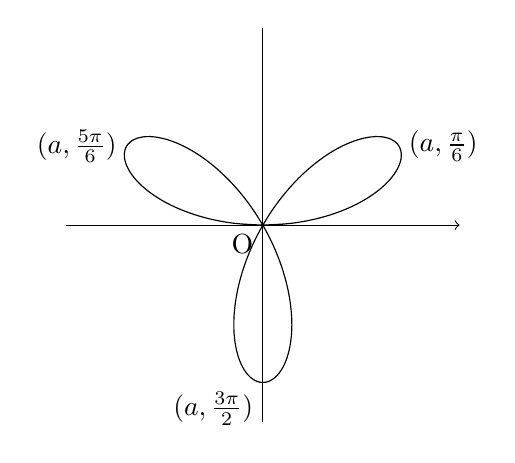
\begin{tikzpicture}
    \draw[->] (-2.5,0) -- (2.5,0);
    \draw (0,-2.5) -- (0,2.5);
    \draw (0,0) node[below left] {$\mathrm{O}$} coordinate (O);
    \draw node[right]at({sqrt(3)},1) {$(a,\frac{\pi}{6})$};
    \draw node[left]at(-{sqrt(3)},1) {$(a,\frac{5\pi}{6})$};
    \draw node[below left ] at(0,-2) {$(a,\frac{3\pi}{2})$};
    \draw plot[domain=0:{2*pi},samples=100, variable=\t, smooth](\t r:{2*sin(3*\t r)});
    \end{tikzpicture} 
    }

    \subsection*{p68:問26-(2)}
\addcontentsline{toc}{subsection}{\texorpdfstring{p68:問26-(2)}{p68:問26-(2)}}

\scalebox{0.8}[0.8]{
    \begin{tikzpicture}
    \draw[->] (-4,0) -- (7,0);
    \draw (0,-6)--(0,4);
    \draw (0,0) node[below left] {$\mathrm{O}$} coordinate (O);
    \draw plot[domain=0:{2*pi},samples=100, variable=\t, smooth](\t r:\t);
    \end{tikzpicture} 
}

\subsection*{p68:1-(1)}
\addcontentsline{toc}{subsection}{\texorpdfstring{p68:1-(1)}{p68:1-(1)}}

\begin{tleftbar}
    計算すると,
    \begin{align*} 
        \frac{d}{dx} \left ( \frac{1}{2} \log \abs{\frac{1+x}{1-x}} \right) & =\frac{1}{2} \frac{d}{dx} (\log  \abs{1+x}- \log \abs{1-x} ) \\
        & = \frac{1}{2} \left (\frac{1}{1+x}+\frac{1}{1-x} \right ) \\
        & = \frac{1}{(1+x)(1-x)}
    \end{align*} 
    となる.
\end{tleftbar}


\subsection*{p68:1-(8)}
\addcontentsline{toc}{subsection}{\texorpdfstring{p68:1-(8)}{p68:1-(8)}}

\begin{tleftbar}
    計算すると,
    \begin{align*} 
       \frac{d}{dx} \left ( \log \sqrt{\frac{1-\cos x}{1+\cos x}} \right) & = \frac{1}{2} \frac{\left (\dfrac{1-\cos x}{1+\cos x} \right)'}{ \dfrac{1-\cos x}{1+\cos x} } \\
       & = \frac{\sin x}{1-\cos ^2 x}\\
       & = \frac{1}{\sin x}
    \end{align*}
    となる.
\end{tleftbar}


\subsection*{p68:2-(1)}
\addcontentsline{toc}{subsection}{\texorpdfstring{p68:2-(1)}{p68:2-(1)}}

\begin{tleftbar}
    計算すると,
    \begin{align*} 
        \frac{dy}{dx} & = \frac{ dy / dt}{dx /dt} \\
        & = \frac{a\cosh t}{a \sinh t} \\
        & = \frac{\cosh t}{\sinh t} \\
        & =\frac{1}{\tanh t}
    \end{align*} 
    である.

    また,
    \begin{align*} 
        \frac{d^2 y}{d x^2} & = \frac{d}{dt} \left (\frac{dy}{dx} \right ) \cdot  \frac{dt}{dx} \\
        & = \frac{d}{dt} \left ( \frac{1}{\tanh t} \right)\cdot \frac{1}{a\sinh t} \\
        & = -\frac{1}{\sinh^2 t} \cdot \frac{1}{a \sinh t} \\
        & = -\frac{1}{a\sinh ^3t}
    \end{align*} 
    となる.
\end{tleftbar}

\subsection*{p68:2-(2)}
\addcontentsline{toc}{subsection}{\texorpdfstring{p68:2-(2)}{p68:2-(2)}}

\begin{tleftbar}
    計算すると,
    \begin{align*} 
        \frac{dy}{dx} & = \frac{ dy / dt}{dx /dt} \\
        & = \frac{ 3a \sin ^2 t \cos t)}{3a \cos ^2 t (-\sin t)} \\
        & =\frac{\sin t}{-\cos  t} \\
        & =-\tan t
    \end{align*} 
    である.

    また,
    \begin{align*} 
        \frac{d^2 y}{d x^2} & = \frac{d}{dt} \left (\frac{dy}{dx} \right ) \cdot  \frac{dt}{dx} \\
        & = \frac{d}{dt} ( -\tan t)\cdot \frac{1}{3a \cos ^2 t (-\sin t)} \\
        & = -\frac{1}{\cos ^2 t }\cdot \frac{1}{3a \cos ^2 t (-\sin t)} \\
        & = -\frac{1}{3a \cos ^4 t \sin t}
    \end{align*} 
    である.
\end{tleftbar}


\subsection*{p68:3-(1)}
\addcontentsline{toc}{subsection}{\texorpdfstring{p68:3-(1)}{p68:3-(1)}}

\begin{tleftbar}
    まず,
    \[
        \cos x + \cos 2x = \frac{\cos 3x + \cos x}{2}
    \]
    なので,
    \[
        y^{(n)} = \frac{1}{2} \left  ( 3^n \cos \left (3x + \frac{n \pi}{2} \right)+ \cos \left (x + \frac{n \pi}{2}\right) \right)
    \]
    である.
\end{tleftbar}


\subsection*{p69:4-(1)}
\addcontentsline{toc}{subsection}{\texorpdfstring{p69:4-(1)}{p69:4-(1)}}

\begin{tleftbar}
    \[
        f(x)=(1+x)^\alpha - (1+\alpha x)
    \]
    とおくと,
    \begin{align*} 
        &f'(x) = \alpha (1+x)^{\alpha -1} - \alpha \\
        & f''(x)= \alpha(\alpha-1) (1+x)^{\alpha -2} >0
    \end{align*} 
    となるため,$f'(-1)= 0$と併せると,$x>-1$のとき$f'(x) >0$である.

    よって,$ x>-1$のとき,$f(x)$は単調に増加し,
    \[
        f(-1)=0-1+\alpha >0
    \]
    であることをふまえると,$x>-1$のとき$f(x)>0$である.

    よって,$x>-1$のとき,
    \begin{align*} 
        & (1+x)^\alpha - (1+\alpha x)>0 \\
        & (1+x)^\alpha > (1+\alpha x)
    \end{align*} 
    である.
\end{tleftbar}


\subsection*{p69:4-(2)}
\addcontentsline{toc}{subsection}{\texorpdfstring{p69:4-(2)}{p69:4-(2)}}


\begin{tleftbar}
    \[
        f(x)=(1+x)^\alpha - (1+\alpha x)
    \]
    とおくと,
    \begin{align*} 
        &f'(x) = \alpha (1+x)^{\alpha -1} - \alpha \\
        & f''(x)= \alpha(\alpha-1) (1+x)^{\alpha -2} <0
    \end{align*} 
    となるため,$f'(-1)= 0$と併せると,$x>-1$のとき$f'(x) <0$である.

    よって,$ x>-1$のとき,$f(x)$は単調に減少し,
    \[
        f(-1)=0-1+\alpha <0
    \]
    であることをふまえると,$x>-1$のとき$f(x)<0$である.

    よって,$x>-1$のとき,
    \begin{align*} 
        & (1+x)^\alpha - (1+\alpha x)<0 \\
        & (1+x)^\alpha < (1+\alpha x)
    \end{align*} 
    である.
\end{tleftbar}


\subsection*{p69:4-(3)}
\addcontentsline{toc}{subsection}{\texorpdfstring{p69:4-(3)}{p69:4-(3)}}


グラフは下図のようになる.
    \begin{figure}[htbp]
\scalebox{1.1}[1.1]{
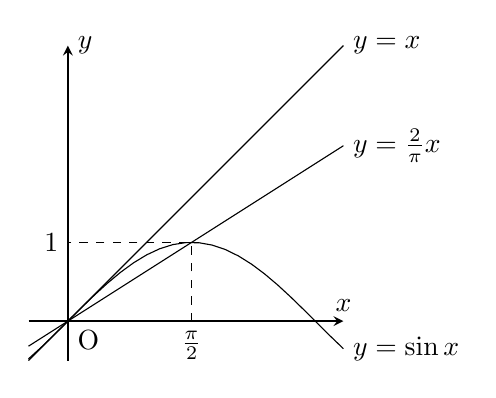
\begin{tikzpicture}
\draw[->,>=stealth,semithick](-0.5,0)--(3.5,0)node[above]{$x$};%x軸
\draw[->,>=stealth,semithick](0,-0.5)--(0,3.5)node[right]{$y$};%y軸
\draw(0,0)node[below right]{O};%原点
\draw[dashed](pi/2,0)node[below]{$\frac{\pi}{2}$}--(pi/2,1)--(0,1)node[left]{$1$};%点(1,1)
\draw[domain=-0.5:3.5]plot(\x,{2*\x/pi})node[right]{$y=\frac{2}{\pi} x$};
\draw[domain=-0.5:3.5]plot(\x,{sin(\x r)})node[right]{$y=\sin x$};
\draw[domain=-0.5:3.5]plot(\x,\x)node[right]{$y=x$};
\end{tikzpicture} }
\end{figure}

図より,$0<x<\pi/2$のとき
\[
    \frac{2}{\pi} x < \sin x < x 
\]
である.


\subsection*{p69:4-(4)}
\addcontentsline{toc}{subsection}{\texorpdfstring{p69:4-(4)}{p69:4-(4)}}

\[
    f(x)= x - \sin x
\]
とおくと,$f'(x)= -\cos x+1>0$となるため,$f$は$x>0$で単調に増加する.

$f(0)=0$であることを考慮すると,
$x>0$のとき$f(x)>0$であるから,
\[
    x>\sin x
\]
となる.

また,
\[
    g(x)=\sin x - \left ( x-\frac{x^3}{6!} \right)
\]
とおくと,
\begin{align*}
    &g'(x)= \cos x -\left  (1-\frac{x^2}{2} \right) \\
    &g''(x)= -\sin x +x >0
\end{align*}
となるため,$g'(x)$は$x>0$で単調に増加する.

ここで,$g'(0)=0$であることから,$x>0$のとき$g'(x) >0$となり,
$g(x)$は$x>0$で単調に増加する.

これと$g(0)=0$であることを考慮すると,$x>0$のとき$g(x)>0$であり,
\[
    \sin x > x-\frac{x^3}{6!} 
\]
となる.

グラフは下図のようになる.
    \begin{figure}[htbp]
\scalebox{1.1}[1.1]{
\begin{tikzpicture}
\draw[->,>=stealth,semithick](-0.5,0)--(3.5,0)node[above]{$x$};%x軸
\draw[->,>=stealth,semithick](0,-0.5)--(0,3.5)node[right]{$y$};%y軸
\draw(0,0)node[below right]{O};%原点
\draw[domain=-0.5:3.3]plot(\x,{-{pow( \x ,3 )}/6 +\x})node[right]{$y=x-\frac{x^3}{3!}$};
\draw[domain=-0.5:3.3]plot(\x,{sin(\x r)})node[below right]{$y=\sin x$};
\draw[domain=-0.5:3.3]plot(\x,\x)node[right]{$y=x$};
\end{tikzpicture} }
\end{figure}


\subsection*{p69:4-(5)}
\addcontentsline{toc}{subsection}{\texorpdfstring{p69:4-(5)}{p69:4-(5)}}

まず,
\[
    f(x)= \cos x - \left ( 1-\frac{x^2}{2!} \right)
\]
とおく.微分すると,
\begin{align*}
   &  f'(x)= -\sin x +x \\
   & f''(x) = -\cos x +1 >0
\end{align*}
となるため,$f'$は$x>0$で単調増加である.

さらに$f'(0)=0$であることをふまえると,$x>0$のとき$f'(x)>0$であるから,$f$は$x>0$で単調増加であり,
$f(0)=0$だから,
\[
    \cos x > 1-\frac{x^2}{2!} 
\]
である.

次に,

\[
    g(x)= \left ( 1-\frac{x^2}{2!} + \frac{x^4}{4!} \right) - \cos x
\]
とおくと,
\begin{align*} 
    & g'(x)= -x + \frac{x^3}{3!} + \sin x \\
    & g''(x) = -1 + \frac{x^2}{2!} + \cos x \\
    & g'''(x) = x -\sin x \\
    & g''''(x)= 1 -\cos x >0
\end{align*} 
であることから,同様の議論により,
\[
     1-\frac{x^2}{2!} + \frac{x^4}{4!} >\cos x
\]
となる.

以上の議論により,
\[
    1-\frac{x^2}{2!}  < \cos x <  1-\frac{x^2}{2!} + \frac{x^4}{4!}
\]
である.

\begin{figure}[htbp]
    \scalebox{1.1}[1.1]{
    \begin{tikzpicture}
    \draw[->,>=stealth,semithick](-0.5,0)--(3.5,0)node[above]{$x$};%x軸
    \draw[->,>=stealth,semithick](0,-3.5)--(0,1.5)node[right]{$y$};%y軸
    \draw(0,0)node[below right]{O};%原点
    \draw[domain=-0.5:3.2]plot(\x,{-{pow( \x ,2 )}/2 +1})node[right]{$y=1-\frac{x^2}{2!}$};
    \draw[domain=-0.5:3.2]plot(\x,{cos(\x r)})node[below]{$y=\cos x$};
    \draw[domain=-0.5:3.2]plot(\x,{-pow( \x ,2 )/2 + 1 + pow( \x ,4 )/(24)})node[below right]{$y=1-\frac{x^2}{2!}+\frac{x^4}{4!}$};
    \end{tikzpicture} }
    \end{figure}

    \subsection*{p69:5-(1)}
    \addcontentsline{toc}{subsection}{\texorpdfstring{p69:5-(1)}{p69:5-(1)}}

    \begin{tleftbar}
        まず,$\lim_{x \to 0} (\tan x -x)=0$,$\lim_{x \to 0} x^3 =0$となるため,
        ロピタルの定理が適用でき,
        \begin{align*}
            &\lim_{x \to 0} \frac{\tan x -x }{x^3}  \\
            =&  \lim_{x \to 0} \frac{\tan ^2 x }{3x^2} \\
            =&\lim_{x \to 0} \frac{2\tan x (\tan ^2 x +1)}{6x} \\
            =&  \lim_{x \to 0} \frac{6\tan ^2 x (\tan^2 x  +1) + 2 (\tan ^2 x +1)}{6} \\
            =& \frac{2}{6} \\
            =& \frac{1}{3}
        \end{align*}
        となる.
    \end{tleftbar}



    \subsection*{p69:5-(2)}
    \addcontentsline{toc}{subsection}{\texorpdfstring{p69:5-(2)}{p69:5-(2)}}

    \begin{tleftbar}
        まず,
        \[
            \frac{1}{x^2}-\frac{1}{\sin ^2 x} = \frac{\sin ^2 x-x^2}{x^2 \sin ^2 x}
        \]
        と変形でき,$\lim_{x \to 0} (\sin ^2 x-x^2)=0$,$\lim_{x \to 0} x^2 \sin ^2 x=0$であるから,ロピタルの定理が適用でき

        \begin{align*} 
            &\lim_{x \to 0} \frac{\sin ^2 x - x^2}{x^2 \sin ^2 x} \\
            =&\lim_{x \to 0} \frac{\sin 2x - 2x}{2x \sin ^2 x + x^2 \sin 2 x} \\
            =& \lim_{x \to 0} \frac{2\cos 2x -2}{2 \sin ^2 x + 4x \sin 2x +2x^2 \cos 2x} \\
            =& \lim_{x \to 0} \frac{-4\sin 2x}{2\sin 2x + 12x\cos 2x  -2x^2 \sin 2x } \\
            =& \frac{-4}{0+12+0} \\
            =& -\frac{1}{3}
        \end{align*} 
        となる.
    \end{tleftbar}


    \subsection*{p69:5-(3)}
    \addcontentsline{toc}{subsection}{\texorpdfstring{p69:5-(3)}{p69:5-(3)}}

    \begin{tleftbar}
        $\lim_{x \to 0} (e^x - e^{\sin x})=0$,$\lim_{x \to 0} x^3 =0$であるから,ロピタルの定理が適用でき
        \begin{align*} 
            & \lim_{x \to 0} \frac{e^x - e^{\sin x}}{x^3} \\
            =& \lim_{x \to 0} \frac{e^x - e^{\sin x} \cos x}{3x^2} \\
            =& \lim_{x \to 0} \frac{e^x - e^{\sin x } \cos^2 x + e^{\sin x} \sin x}{6x} \\
            =& \lim_{x \to 0} \frac{e^x - e^{\sin x} \cos ^3 x +\dfrac{3}{2}e^{\sin x} \sin 2x  + e^{\sin x} \cos x}{6} \\
            =&\frac{1-1^3 +0 +1}{6} \\
            =&\frac{1}{6}
        \end{align*} 
        である.
    \end{tleftbar}

    \subsection*{p69:5-(7)}
    \addcontentsline{toc}{subsection}{\texorpdfstring{p69:5-(7)}{p69:5-(7)}}

    \begin{tleftbar}
        自然対数をとって考えると,
        \[
            \lim_{x \to \infty} \log x^{1/x}  = \lim_{x \to 0} \frac{\log x}{x} 
        \]
        であり,$\lim_{x \to \infty} \log x = \infty$,$\lim_{x \to \infty} x = \infty$であるから,
        ロピタルの定理が適用でき,
        \begin{align*} 
            \lim_{x \to \infty} \frac{\log x}{x}  & = \lim_{ x \to \infty} \frac{1/x}{1} \\
            & = 0 
        \end{align*} 
        となるため,
        \begin{align*}
            \lim_{x \to \infty} x^{1/x} &= e^0  \\
            & =1 
        \end{align*}
        である.
    \end{tleftbar}

\section*{第3章:不定積分と微分方程式}
\addcontentsline{toc}{section}{\texorpdfstring{第3章:不定積分と微分方程式}{第3章:不定積分と微分方程式}}


\subsection*{p77:問1-(1)}
\addcontentsline{toc}{subsection}{\texorpdfstring{p77:問1-(1)}{p77:問1-(1)}}

\begin{tleftbar}
    計算すると,
    \begin{align*} 
       \int  x^2 e^{-x} \, dx & = x^2 (-e^{-x})-\int 2x \cdot (-e^{-x})\, dx \\
       & =-x^2 e^{-x} -\left (2xe^{-x}-\int 2 \cdot e^{-x} \, dx \right) \\
       & = -x^2 e^{-x} - 2xe^{-x} -2e^{-x}+\mathrm{Constant.}
    \end{align*} 
    となる.
\end{tleftbar}


\subsection*{p77:問1-(2)}
\addcontentsline{toc}{subsection}{\texorpdfstring{p77:問1-(2)}{p77:問1-(2)}}



\begin{tleftbar}
    計算すると,
    \begin{align*} 
       \int  x^3 \log x \, dx & = \frac{x^4}{4} \log x - \int \frac{x^4}{4} \cdot \frac{1}{x} \, dx \\
       & = \frac{x^4\log x}{4} - \frac{x^4}{16} + \mathrm{Constant.}
    \end{align*}
        となる.
\end{tleftbar}


\subsection*{p77:問1-(3)}
\addcontentsline{toc}{subsection}{\texorpdfstring{p77:問1-(3)}{p77:問1-(3)}}

\begin{tleftbar}
    \[
        \frac{1}{\sqrt{x}+\sqrt{x+1}} = \sqrt{x+1}-\sqrt{x}
    \]
    であるから,
    \begin{align*} 
        \int \frac{1}{\sqrt{x}+\sqrt{x+1}} \, dx & = \int ( (x+1)^\frac{1}{2} -x^\frac{1}{2} ) \, dx \\
        & = \frac{2}{3} ( (x+1)^\frac{3}{2} - x^\frac{3}{2} ) + \mathrm{Constant.}
    \end{align*} 
    となる.
\end{tleftbar}


\subsection*{p77:問1-(5)}
\addcontentsline{toc}{subsection}{\texorpdfstring{p77:問1-(5)}{p77:問1-(5)}}

\begin{tleftbar}
    まず,
    \begin{align*} 
        \tan ^2 x &= \frac{\sin^2 x}{\cos ^2 x} \\
        & = \frac{1}{\cos ^2 x}-1
    \end{align*} 
    であるから,
    \begin{align*} 
        \int \tan ^2 x \, dx & = \int \left (  \frac{1}{\cos ^2 x}-1 \right) \\
        & = \tan x -x +\mathrm{Constant.}
    \end{align*} 
    となる.
\end{tleftbar}

\subsection*{p77:問1-(6)}
\addcontentsline{toc}{subsection}{\texorpdfstring{p77:問1-(6)}{p77:問1-(6)}}

\begin{tleftbar}
    計算すると,
    \begin{align*} 
        \int \frac{\log x}{x} \, dx & =\int (\log x) (\log x)' \, dx \\
        & = \frac{1}{2} (\log x)^2 + \mathrm{Constant.}
    \end{align*} 
    となる.
\end{tleftbar}


\subsection*{p77:問1-(7)}
\addcontentsline{toc}{subsection}{\texorpdfstring{p77:問1-(7)}{p77:問1-(7)}}

\begin{tleftbar}
    計算すると,
    \begin{align*} 
        \int \frac{x}{\sqrt{1+x^2}} \, dx & = \int \frac{\frac{1}{2}(1+x^2)'}{(1+x^2)^\frac{1}{2}} \, dx \\
        & = \sqrt{1+x^2}+\mathrm{Constant.}
    \end{align*}
    となる.
\end{tleftbar}

\subsection*{p77:問1-(8)}
\addcontentsline{toc}{subsection}{\texorpdfstring{p77:問1-(8)}{p77:問1-(8)}}

\begin{tleftbar}
    まず,
    \[
        \cos ^3 x = \cos x (1-\sin ^2 x) = \cos x - \sin ^2 x \cos x 
    \]
    と変形できるので,
    \begin{align*} 
        \int \cos ^3 x \, dx & = \int (\cos x - \sin ^2 x (\sin x)' ) \, dx \\
        & = \sin x -\frac{\sin ^3 x}{3} + \mathrm{Constant.}
    \end{align*}
        となる.
\end{tleftbar}


\subsection*{p77:問1-(8)}
\addcontentsline{toc}{subsection}{\texorpdfstring{p77:問1-(8)}{p77:問1-(8)}}

\begin{tleftbar}
    計算すると,
    \begin{align*} 
        \int x e^{x^2} \, dx & = \int \frac{(x^2)' e^{x^2}}{2} \, dx \\
        & = \frac{e^{x^2}}{2}+\mathrm{Constant.}
    \end{align*} 
    となる.
\end{tleftbar}


\subsection*{p77:問1-(9)}
\addcontentsline{toc}{subsection}{\texorpdfstring{p77:問1-(9)}{p77:問1-(9)}}

\begin{tleftbar}
    計算すると,
    \begin{align*} 
        \int \frac{e^x-e^{-x}}{e^x+e^{-x}}  \, dx & = \int \frac{(e^x+e^{-x})'}{e^x+e^{-x}} \, dx \\
        & = \log (e^x + e^{-x})+\mathrm{Constant.}
    \end{align*} 
    となる.
\end{tleftbar}


\subsection*{p77:問2}
\addcontentsline{toc}{subsection}{\texorpdfstring{p77:問2}{p77:問2}}

\begin{tleftbar}
    $I+J$を考えると
    \begin{align*} 
        I + J & = \int \frac{\sin x+\cos x}{\sin x + \cos x} \, dx \\
        & = \int \, dx \\
        & = x
    \end{align*} 
    である.

    また,$ J-I$を考えると,
    \begin{align*} 
        J - I & = \int \frac{\cos x -\sin x}{\sin x + \cos x} \, dx \\
        & = \int \frac{(\sin x + \cos x)'}{\sin x + \cos x} \, dx \\
        & = \log \abs{\sin x+\cos x}
    \end{align*}
    であるから,
    \[
        I = \frac{1}{2}(x- \log \abs{\sin x + \cos x}),\quad J = \frac{1}{2} ( x + \log \abs{\sin x + \cos x})
    \]
    である.
\end{tleftbar}

\subsection*{p81:問6-(1)}
\addcontentsline{toc}{subsection}{\texorpdfstring{p81:問6-(1)}{p81:問6-(1)}}

\begin{tleftbar}
    $ \tan (x/2)=t$とおくと,
    \[
        \cos x = \frac{1-t^2}{1+t^2} ,\quad dx = \frac{2dt}{1+t^2}
    \]
    なので,
    \begin{align*} 
    \int \frac{dx}{\cos x} & = \int \frac{2}{1+t^2} \cdot \frac{1+t^2}{1-t^2} \, dt \\
    & = \int \frac{2dt}{1-t^2} \\
    & = \int \left ( \frac{1}{1-t}-\frac{1}{1+t} \right) \, dt\\
    & = \log \abs{\frac{1-t}{1+t}} + \mathrm{Constant.} \\
    & = \log \abs{\frac{1-\tan (x/2)}{1+\tan (x/2)}}+\mathrm{Constant.} 
    \end{align*}
    となる.
\end{tleftbar}

\begin{tleftbar}
    $ \sin x = t$とおくと,$\frac{dt}{dx}= \cos x$であり,
    \begin{align*} 
        \int \frac{1}{\cos x}\, dx & = \int \frac{1}{1-t^2} \, dt \\
        & = \frac{1}{2} \log \abs{\frac{1-\sin x}{1+\sin x}} + \mathrm{Constant.}
    \end{align*}
    となる.
\end{tleftbar}


\subsection*{p83:問7-(1)}
\addcontentsline{toc}{subsection}{\texorpdfstring{p83:問7-(1)}{p83:問7-(1)}}

\begin{tleftbar}
    まず,$ \sqrt{x^2+1}=t$とおくと,$x^2 + 1 = t^2$により,$ t dt = x dx $である.

    これを用いると,
    \begin{align*}
        \int \frac{1}{x\sqrt{x^2+1}} \, dx & = \int \frac{1}{(t^2-1)} \, dt \\
        & = \int  \frac{1}{2} \left (\frac{1}{t-1}-\frac{1}{t+1} \right ) \, dt \\
        & = \frac{1}{2} \log \abs{\frac{t-1}{t+1}} + \mathrm{Constant.} \\
        & = \frac{1}{2} \log \abs{\frac{\sqrt{x^2+1}-1}{\sqrt{x^2+1}+1}} +\mathrm{Constant.} 
    \end{align*}
    となる.
\end{tleftbar}


\subsection*{p98:演習問題1-(1)}
\addcontentsline{toc}{subsection}{\texorpdfstring{p98:演習問題1-(1)}{p98:演習問題1-(1)}}

\begin{tleftbar}
    \begin{align*} 
        \int \log (1+x)\, dx & = (1+x) \log (1+x) - \int (1+x) \cdot (\log (1+x))' \, dx \\
        & = (1+x) \log (1+x) - \int \, dx \\
        & = (1+x) \log (1+x) - x +\mathrm{Constant.}
    \end{align*} 
\end{tleftbar}


\subsection*{p98:演習問題1-(2)}
\addcontentsline{toc}{subsection}{\texorpdfstring{p98:演習問題1-(2)}{p98:演習問題1-(2)}}

\begin{tleftbar}
    $\alpha \ne -1 , -2$のとき,
    \begin{align*} 
        \int x (x+1)^{\alpha} \, dx & = \frac{x}{\alpha +1} (x+1)^{\alpha+1} -\int \frac{(x+1)^{\alpha+1}}{\alpha +1} (x+1)^{\alpha+1} \, dx \\
        & = \frac{x}{\alpha +1} (x+1)^{\alpha+1} - \frac{(x+1)^{\alpha +2}}{(\alpha+1)(\alpha+2)}+ \mathrm{Constant.}
    \end{align*}
    $\alpha =-1$のとき,
    \begin{align*} 
        \int \frac{x}{x+1} \, dx & = \int \left ( 1 - \frac{1}{x+1} \right) \, dx \\
        & = x - \log \abs{x+1} + \mathrm{Constant.}
    \end{align*} 
    $ \alpha = -2$のとき,
    \begin{align*} 
        \int \frac{x}{(x+1)^2} \, dx & = \int \frac{t-1}{t^2} \, dt \\
        & = \int \left (\frac{1}{t}-\frac{1}{t^2} \right) \, dt \\
        & = \log \abs{x+1} +\frac{1}{x+1} + \mathrm{Constant.} 
    \end{align*} 
\end{tleftbar}


\subsection*{p98:演習問題1-(7)}
\addcontentsline{toc}{subsection}{\texorpdfstring{p98:演習問題1-(7)}{p98:演習問題1-(7)}}

\begin{tleftbar}
    $ t = e^x$とおくと,$\frac{dt}{dx}=e^x$であり,
    \begin{align*} 
        \int \frac{e^x}{\sqrt{e^{2x}-1}} \, dx & = \int \frac{1}{\sqrt{t^2-1}} \, dt \\
        & = \log \abs{t+\sqrt{t^2-1}} + \mathrm{Constant.} \\
        & = \log \abs{e^x +\sqrt{e^{2x}-1}}+\mathrm{Constant.}
    \end{align*} 
    となる.
\end{tleftbar}



\subsection*{p98:演習問題1-(9)}
\addcontentsline{toc}{subsection}{\texorpdfstring{p98:演習問題1-(9)}{p98:演習問題1-(9)}}

\begin{tleftbar}
\begin{align*} 
    \int (\log x)^3 \, dx & = x (\log x)^3 - \int x \cdot 3 (\log x)^2 \cdot \frac{1}{x} \, dx \\
    & = x(\log x)^3- 3  \int (\log x)^2 \, dx \\
    & = x(\log x)^3 - 3x (\log x)^2 + 3\int x \cdot 2 (\log x )\cdot \frac{1}{x} \, dx \\
    & = x (\log x)^3 - 3x (\log x)^2 + 6 x\log x - 6x+\mathrm{Constant.}
\end{align*} 
となる.
\end{tleftbar}


\subsection*{p98:演習問題2-(5)}
\addcontentsline{toc}{subsection}{\texorpdfstring{p98:演習問題2-(5)}{p98:演習問題2-(5)}}

\begin{tleftbar}
    $\sqrt{x}=t$とおくと,$ x =t^2$であるから$ \frac{dx}{dt}=2t$である.
    よって,
    \begin{align*}
        \int \frac{2t}{t (t^2+1)} \, dt & = \int \frac{2}{t^2+1}\, dt \\
        & = 2 \tan^{-1} t + \mathrm{Constant.}\\
        & = 2 \tan^{-1} \sqrt{x} + \mathrm{Constant.}
    \end{align*} 
    となる.
\end{tleftbar}


\newpage 

\section*{第4章:定積分とその応用}
\addcontentsline{toc}{section}{\texorpdfstring{第4章:定積分とその応用}{第4章:定積分とその応用}}


\subsection*{p103:問1}
\addcontentsline{toc}{subsection}{\texorpdfstring{p103:問1}{p103:問1}}


\begin{tleftbar}
  \begin{proof}
  上方和について証明する.

  $\varDelta$に分点$x^{\ast}$(ただし$ x_{k-1} \leqq x^{\ast} \leqq x_{k}$)を付け加えた分割を$\varDelta '$とする.
  このとき,$ S[\varDelta ']$は,$S[\varDelta]$の
  \[
    M_k (x_k-x_{k-1})
  \]
    の項を
  \[
  M_k' (x^{\ast}-x_{k-1})+M_k ''(x_k - x^{\ast})
  \]
  でおきかえたものとなる.ただしここで
  \[
    M_k ' = \sup \{ f(x) \mid x_{k-1} \leqq x \leqq x^{\ast} \} , \quad M_k '' = \sup \{ f(x) \mid x^\ast \leqq x \leqq x_k \}
  \]
  とおいた.この定義から
  \[
    M_k ' \leqq M_k ,\quad M_k '' \leqq M_k
  \]
  であるから,
  \begin{align*}
    M_k' (x^{\ast}-x_{k-1})+M_k ''(x_k - x^{\ast}) & \leqq M_k (x^{\ast}-x_{k-1})+M_k (x_k - x^{\ast}) \\
    & = M(x_k-x_{k-1})
  \end{align*}
  であるから,$S [\varDelta] \leqq S[ \varDelta']$である.また,分割が複数個のときは同じ操作を繰り返せばよい.
  
  これで上方和について証明でき,下方和についても同様の議論を繰り返して示せる.
\end{proof}
\end{tleftbar}

\newpage 

\subsection*{p128:16-(1),(2)}
\addcontentsline{toc}{subsection}{\texorpdfstring{p128:16-(1),(2)}{p128:16-(1),(2)}}

$\int_{0}^{\pi} x f(\sin x)\, dx $の積分で$x= \pi -t $とすると,
\begin{align*} 
    \int_{0}^{\pi} x f( \sin x) \, dx & = \int_{\pi}^{0} (\pi - t) f(\sin t )\, ( -dt) \\
    & = \pi \int_{0}^{\pi} f(\sin x) \, dx - \int_{0}^{\pi} x f (\sin x)\, dx 
\end{align*} 
となるから,これより左の等式が示される.

右については,
\[
    \int_{0}^{\pi} f(\sin x)\, dx =2 \int_{0}^{\frac{\pi}{2}} f(\sin x) \, dx 
\]
を示せばよいので,
\[
    \int_{0}^{\pi} f(\sin x)\, dx = \int_{0}^{\frac{\pi}{2}} f(\sin x) \, dx + \int_{\frac{\pi}{2}}^{\pi} f(\sin x)\, dx 
\]
の後者の積分において,$ t = \pi -x$とおくと,
\begin{align*}
    \int_{\frac{\pi}{2}}^{\pi} f(\sin x)\, dx &= \int_{\frac{\pi}{2}}^{0} f (\sin t)\, (-dt) \\
    & = \int_{0}^{\frac{\pi}{2}} f (\sin x)\, dx
\end{align*}
となり,これより右の等式が従う.

以上の考察により,
\[
    \int_{0}^{\pi}x f(\sin x)\, dx=\frac{\pi}{2} \int_{0}^{\pi} f(\sin x)\, dx =\pi \int_{0}^{\frac{\pi}{2}} f(\sin x) \, dx 
\]
である.

\begin{thebibliography}{9}
	\bibitem{suita} 理工系の微分積分学:吹田信之・新保経彦
\end{thebibliography}

\end{document}